\documentclass[first=purple,second=dgreen,logo=blueexc]{aaltoslides}

\usepackage[latin9]{inputenc}
\usepackage[T1]{fontenc}
\usepackage{graphicx}
\usepackage{amsfonts,amssymb,amsbsy,amsmath}
\usepackage{tikz}
\usepackage{url}
\usepackage{lastpage}
\usepackage{subfig}
\usepackage{fancyvrb}

\title{Multi-view stereo reconstruction for computer graphics content capture}

\author{Konsta H�ltt�}
\institute{Master's thesis presentation\\
konsta.holtta@aalto.fi}

\aaltofootertext{MVS content capture}{Nov 7, 2014}{\arabic{page}/\pageref{LastPage}\ }

\date{Nov 7, 2014} % \today}

\graphicspath{ {gfx/} }

\newcommand{\kuva}[2]{\begin{figure}[h]
		\includegraphics[width=#1\textwidth]{#2}
\end{figure}}

\newcommand{\simplefig}[4]{%
	\begin{figure}[#1]\begin{center}
		#2
		%\caption{#4}
		%\label{#3}
	\end{center}\end{figure}
}
% \simplegfx{pos-specifier}{width}{filename-and-labelname}{caption}
\newcommand{\simplegfx}[4]{%
	\simplefig{#1}{\includegraphics[width=#2]{#3}}{fig:#3}{#4}
}



\begin{document}

%%%%%%%%%%%%%%%%%%%%%%%%%%%%%%%%%%%%%%%%%%%%%%%%%%%%%%%%%%%%%%%%%%%%%%%%%%%%%%%%%%%%%%%%%%%%%

\aaltotitleframe

%%%%%%%%%%%%%%%%%%%%%%%%%%%%%%%%%%%%%%%%%%%%%%%%%%%%%%%%%%%%%%%%%%%%%%%%%%%%%%%%%%%%%%%%%%%%%

\begin{frame}{Multi-view stereo reconstruction for computer graphics content capture}
	%\kuva{0.5}{}
	(super general pipeline pic here maybe)
	\begin{itemize}
		\item Interest in realistic content in computer graphics
		\item Computer graphics synthesizes images from geometric data
		\item Computer vision analyzes geometry from images
		\item This work: Scanning real life objects using several digital cameras simultaneously
	\end{itemize}
\end{frame}

%%%%%%%%%%%%%%%%%%%%%%%%%%%%%%%%%%%%%%%%%%%%%%%%%%%%%%%%%%%%%%%%%%%%%%%%%%%%%%%%%%%%%%%%%%%%%

\begin{frame}{Contents}
	\begin{itemize}
		\item Intro, motivation
		\item Imaging fundamentals
		\item 3D reconstruction
		\item Scanning rig implementation
		\item Results
		\item Conclusion
	\end{itemize}
\end{frame}

%%%%%%%%%%%%%%%%%%%%%%%%%%%%%%%%%%%%%%%%%%%%%%%%%%%%%%%%%%%%%%%%%%%%%%%%%%%%%%%%%%%%%%%%%%%%%

\begin{frame}{Motivation}
	\kuva{0.8}{ira-eyes}
	{ \centering { \footnotesize Digital Ira (NVIDIA), CGI} \par }
	\begin{itemize}
		\item The processing power of GPUs big and increases
		\item Able to process massive level of detail
		\item Creating content manually tedious, difficult to get right
		\item Digital cameras are really good today
		\item $\Rightarrow$ Scan the geometry and color using digital cameras
	\end{itemize}
\end{frame}

%%%%%%%%%%%%%%%%%%%%%%%%%%%%%%%%%%%%%%%%%%%%%%%%%%%%%%%%%%%%%%%%%%%%%%%%%%%%%%%%%%%%%%%%%%%%%

\begin{frame}{Imaging}
	\center 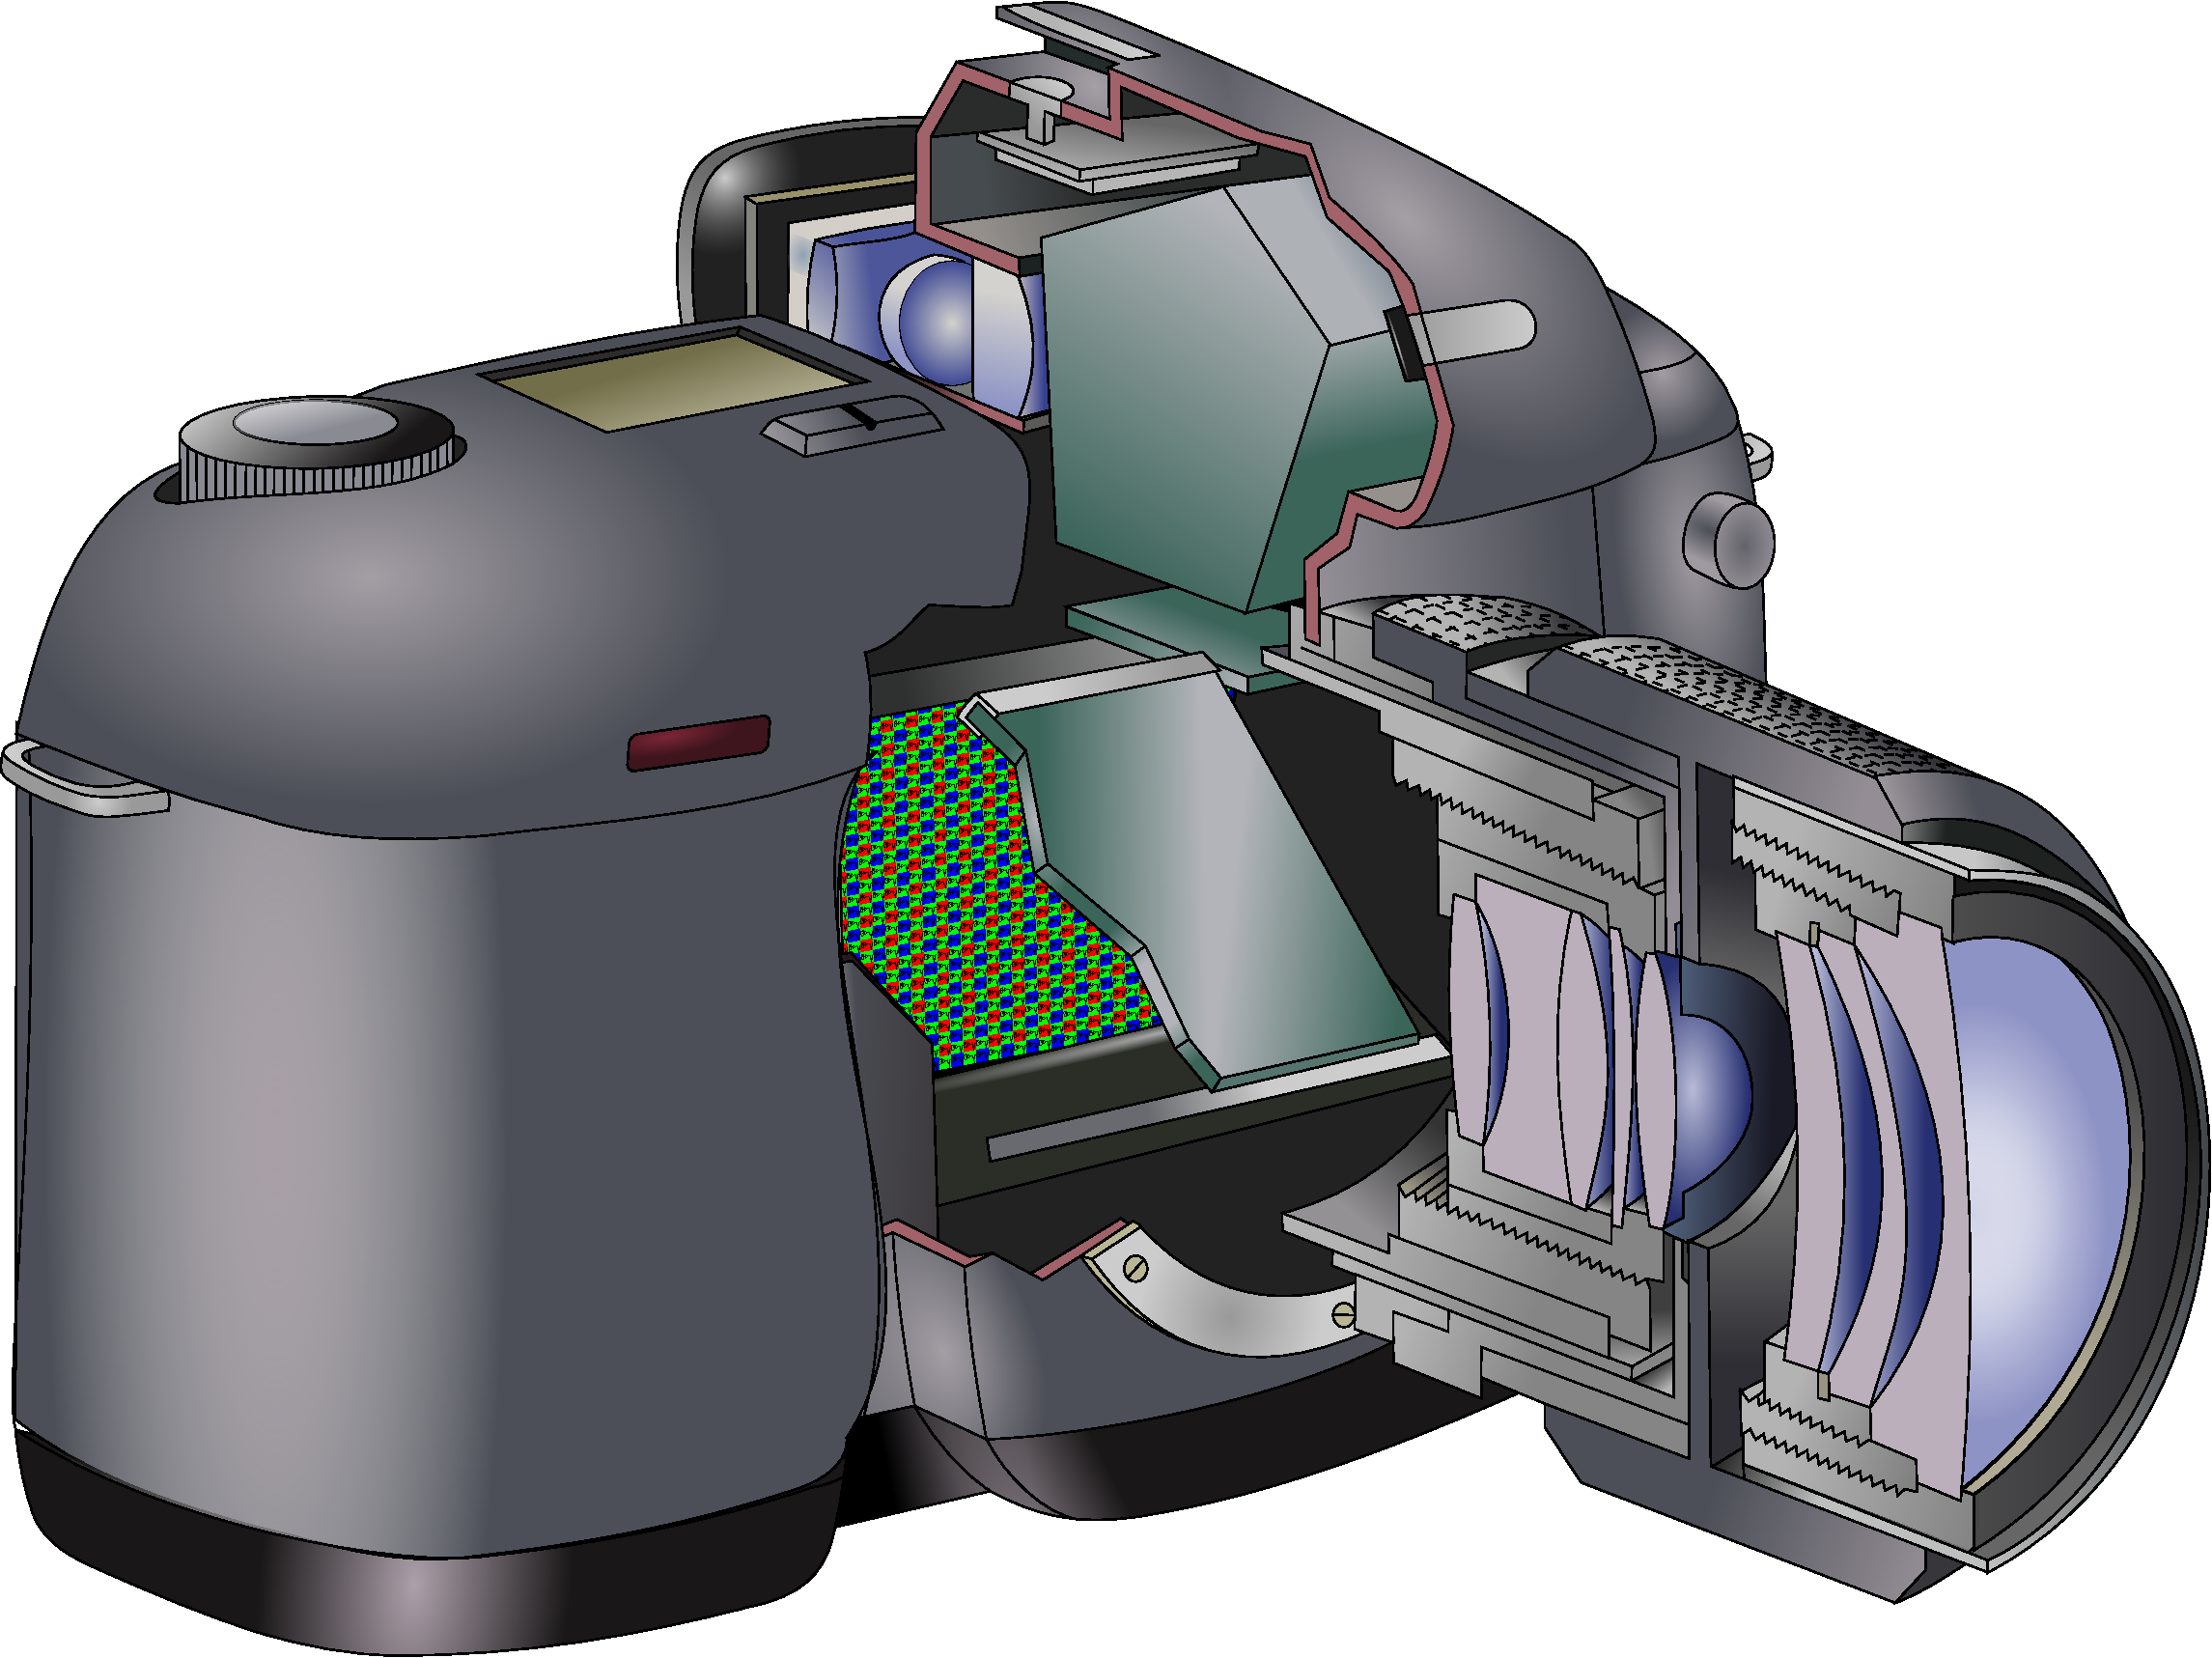
\includegraphics[height=0.4\textheight]{gfx/reflexcamera}
	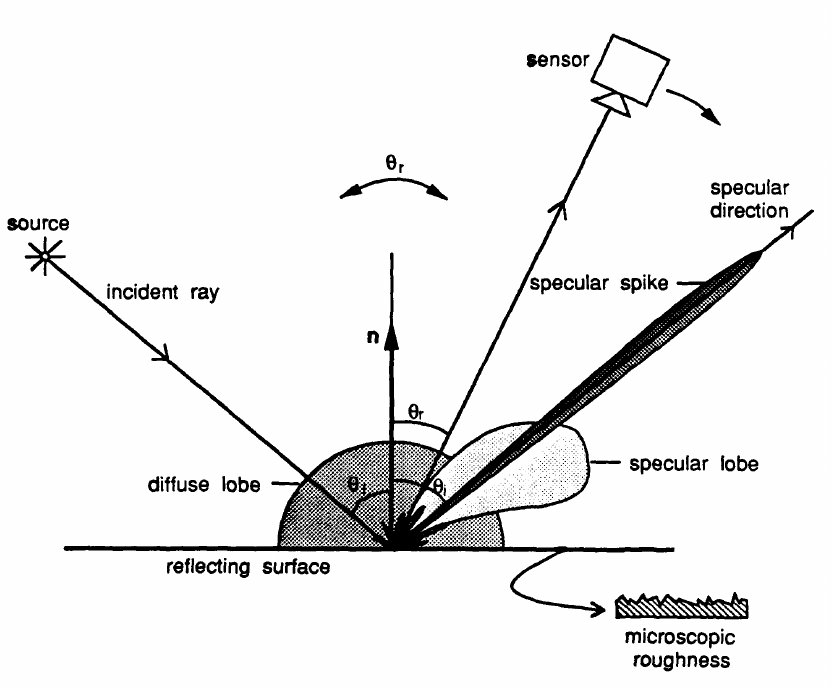
\includegraphics[height=0.4\textheight]{gfx/nayarbrdf}
	\begin{itemize}
		\item Lens systems, geometric distortion, color distortion, depth of field, image resolution, frame rate, motion blur, compression quality, ...
		\item Complete imaging pipeline is complex
		\item Light travels from subject to sensor, to digital file
		\item Assumed uniform lighting, still non-shiny subject
		\item Video = consecutive image frames
	\end{itemize}
\end{frame}

%%%%%%%%%%%%%%%%%%%%%%%%%%%%%%%%%%%%%%%%%%%%%%%%%%%%%%%%%%%%%%%%%%%%%%%%%%%%%%%%%%%%%%%%%%%%%

\begin{frame}{Simplified methods}
	\center 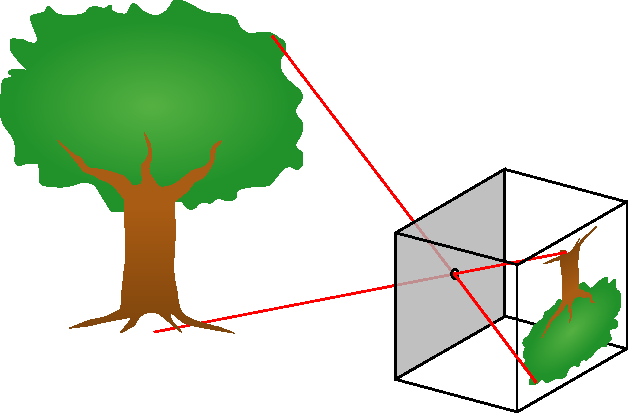
\includegraphics[height=0.4\textheight]{gfx/pinhole-camera}
	\begin{itemize}
		\item Linear camera model, simple optical distortion models, orthogonal problems as separate steps
		\item Assumptions, corner detection, correspondence matching, triangulation, ...
	\end{itemize}
\end{frame}

%%%%%%%%%%%%%%%%%%%%%%%%%%%%%%%%%%%%%%%%%%%%%%%%%%%%%%%%%%%%%%%%%%%%%%%%%%%%%%%%%%%%%%%%%%%%%

\begin{frame}{Video}
	\begin{columns}[c]
	\column{0.5\textwidth}
	\begin{itemize}
		\item Moving subject
		\item Non-flickering lighting
		\item Motion blur
		\item Rolling shutter
		\item Line skipping
		\item Synchronization
	\end{itemize}
	\column{0.5\textwidth}
	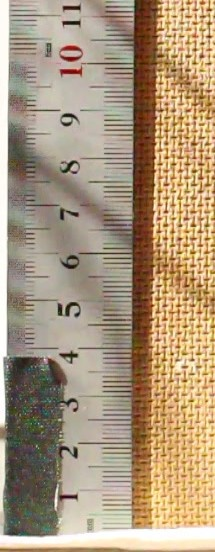
\includegraphics[width=0.3\textwidth]{rollstationary}
	
\includegraphics[width=0.3\textwidth]{roll100}
	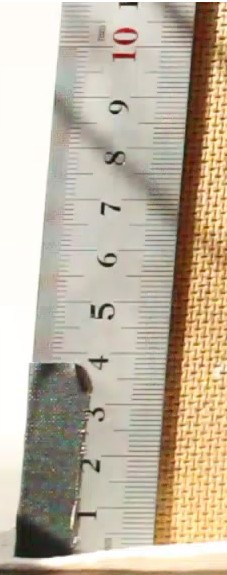
\includegraphics[width=0.3\textwidth]{roll4000}
	\end{columns}
\end{frame}

%%%%%%%%%%%%%%%%%%%%%%%%%%%%%%%%%%%%%%%%%%%%%%%%%%%%%%%%%%%%%%%%%%%%%%%%%%%%%%%%%%%%%%%%%%%%%

\begin{frame}{2D to 3D}
	\begin{itemize}
		\item Camera projection, calibration
		\item Reconstruct 3D geometry $\Leftrightarrow$ apply projection in inverse
		\item Determine scene from multiple viewpoints
	\end{itemize}
\end{frame}

%%%%%%%%%%%%%%%%%%%%%%%%%%%%%%%%%%%%%%%%%%%%%%%%%%%%%%%%%%%%%%%%%%%%%%%%%%%%%%%%%%%%%%%%%%%%%

\begin{frame}{Principle: depth from disparity}
	\begin{columns}[c]
	\column{0.5\textwidth}
	\begin{itemize}
		\item Just simple triangulation, in principle
		\item Two views, two positions in images $\Rightarrow$ 3D position with depth
		\item In practice, many more sophisticated dense algos
		\item Complete pipeline needs to consider everything
	\end{itemize}
	\column{0.5\textwidth}
	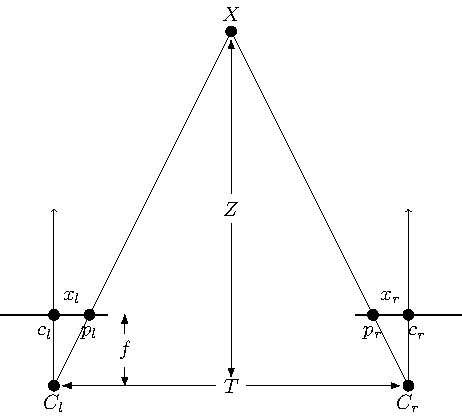
\includegraphics[width=\textwidth]{simplestereo}
	\end{columns}
\end{frame}

%%%%%%%%%%%%%%%%%%%%%%%%%%%%%%%%%%%%%%%%%%%%%%%%%%%%%%%%%%%%%%%%%%%%%%%%%%%%%%%%%%%%%%%%%%%%%

\begin{frame}{(Multi-)Stereo system}
	\hfill 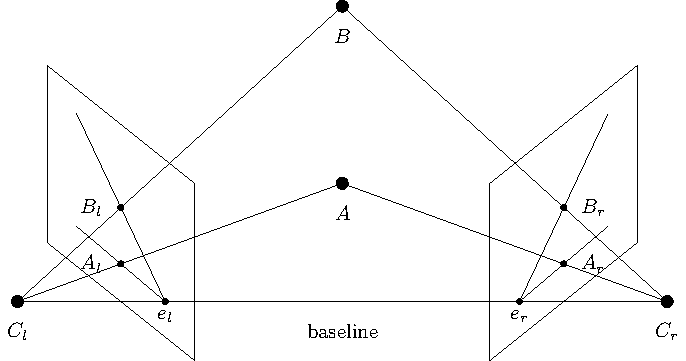
\includegraphics[width=0.5\textwidth]{epigeom}
	\begin{itemize}
		\item Manual or self-calibration
		\item Need camera poses
		\item Reconstruct 3D view
	\end{itemize}
\end{frame}

%%%%%%%%%%%%%%%%%%%%%%%%%%%%%%%%%%%%%%%%%%%%%%%%%%%%%%%%%%%%%%%%%%%%%%%%%%%%%%%%%%%%%%%%%%%%%

\begin{frame}{Reconstruction system}
	\hfill
	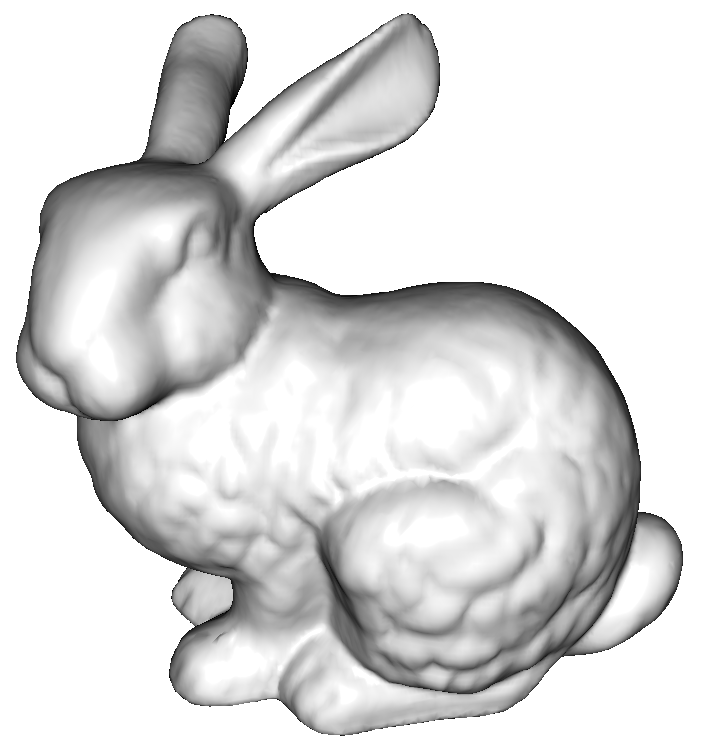
\includegraphics[width=0.3\textwidth]{bunny}
	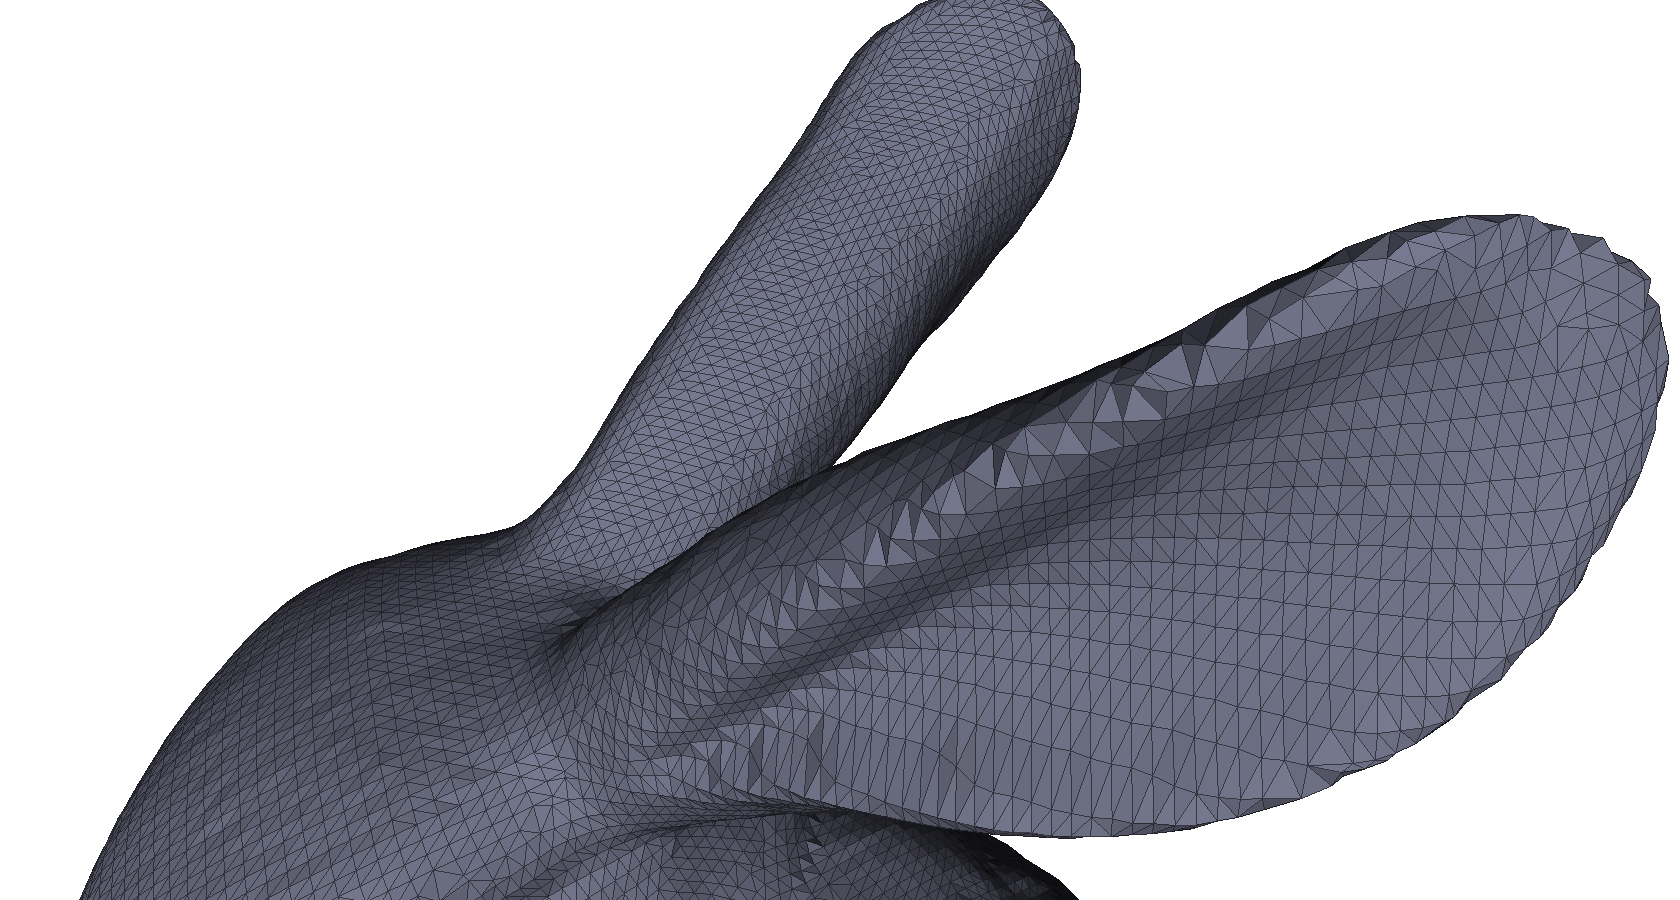
\includegraphics[width=0.6\textwidth]{bunnyear}
	\begin{itemize}
		\item Background theory $\Rightarrow$ construct a reconstruction rig
		\item Acquire a geometric model of a subject
		\item Flexible and general purpose, easy to use
		\item Human head special interest
		\item Heavy study on available hardware and software
	\end{itemize}
\end{frame}

%%%%%%%%%%%%%%%%%%%%%%%%%%%%%%%%%%%%%%%%%%%%%%%%%%%%%%%%%%%%%%%%%%%%%%%%%%%%%%%%%%%%%%%%%%%%%

\begin{frame}{Rig implementation}
	\begin{columns}[c]
	\column{0.5\textwidth}
	\begin{itemize}
		\item 9x Canon EOS 700D DSLR, 50 mm lens
		\item Wired remote trigger tool
		\item auxiliary HW, support SW
		\item Not restricted to any specific reconstruction SW
	\end{itemize}
	\column{0.5\textwidth}
	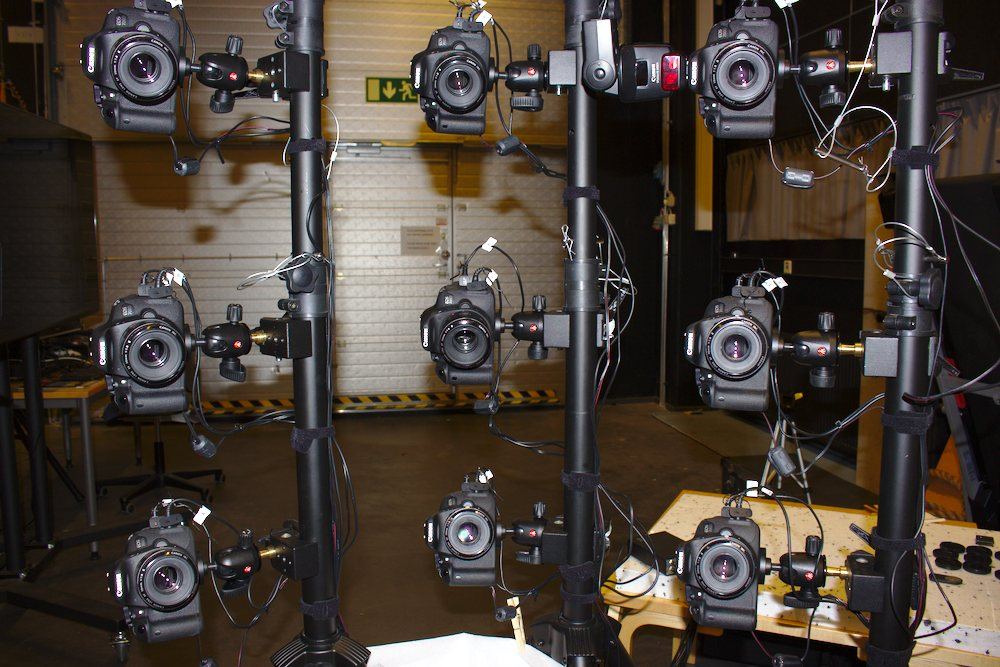
\includegraphics[width=\textwidth]{setupcams}
	\end{columns}
\end{frame}

%%%%%%%%%%%%%%%%%%%%%%%%%%%%%%%%%%%%%%%%%%%%%%%%%%%%%%%%%%%%%%%%%%%%%%%%%%%%%%%%%%%%%%%%%%%%%

\begin{frame}{Remote trigger tool}
	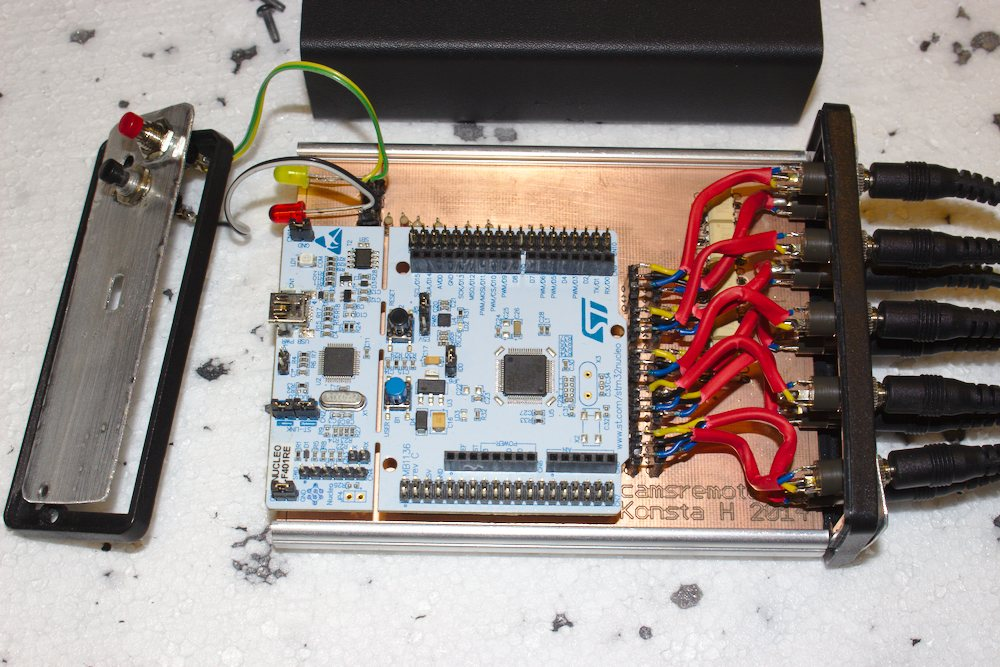
\includegraphics[width=0.5\textwidth]{camsremote}%
	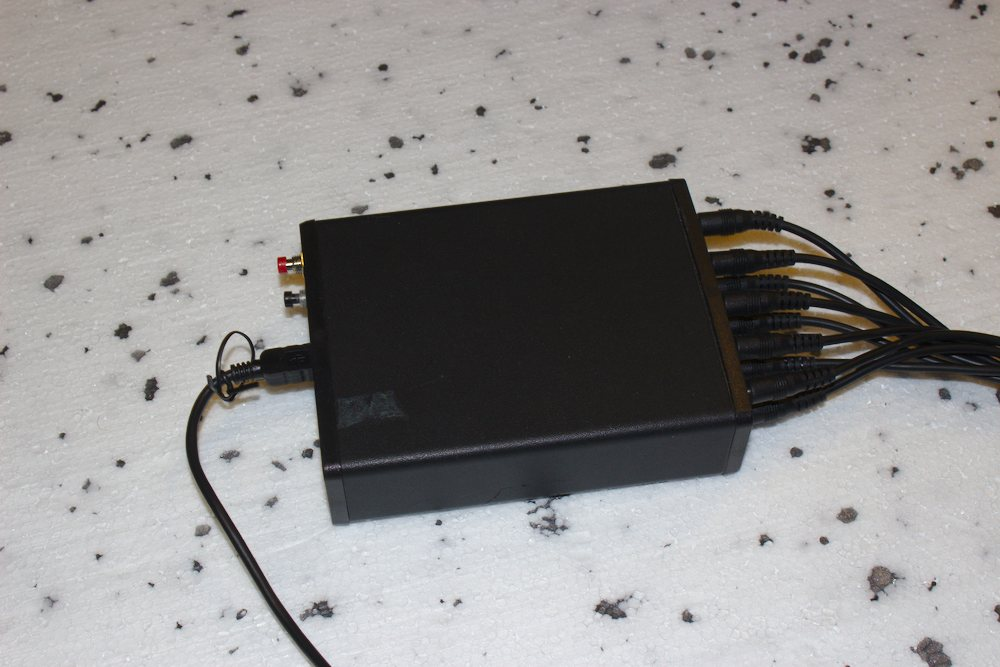
\includegraphics[width=0.5\textwidth]{camsremoteclosed}
	\begin{itemize}
		\item Simultaneous or arbitrary focus and shutter release
		\item Custom built on a microcontroller using wired remote connectors
		\item Commercial tools mostly wireless, expensive
	\end{itemize}
\end{frame}

%%%%%%%%%%%%%%%%%%%%%%%%%%%%%%%%%%%%%%%%%%%%%%%%%%%%%%%%%%%%%%%%%%%%%%%%%%%%%%%%%%%%%%%%%%%%%

\begin{frame}{Software}
	\begin{itemize}
		\item Few options available
		\item Just camera controls, based on \emph{gphoto2}
		\item Generic open source library for cameras
		\item Preview tool, image download, camera configuration, remote shutter
		\item 3D reconstruction development out of scope
	\end{itemize}
\end{frame}

%%%%%%%%%%%%%%%%%%%%%%%%%%%%%%%%%%%%%%%%%%%%%%%%%%%%%%%%%%%%%%%%%%%%%%%%%%%%%%%%%%%%%%%%%%%%%

\begin{frame}{Previewer}
	\center 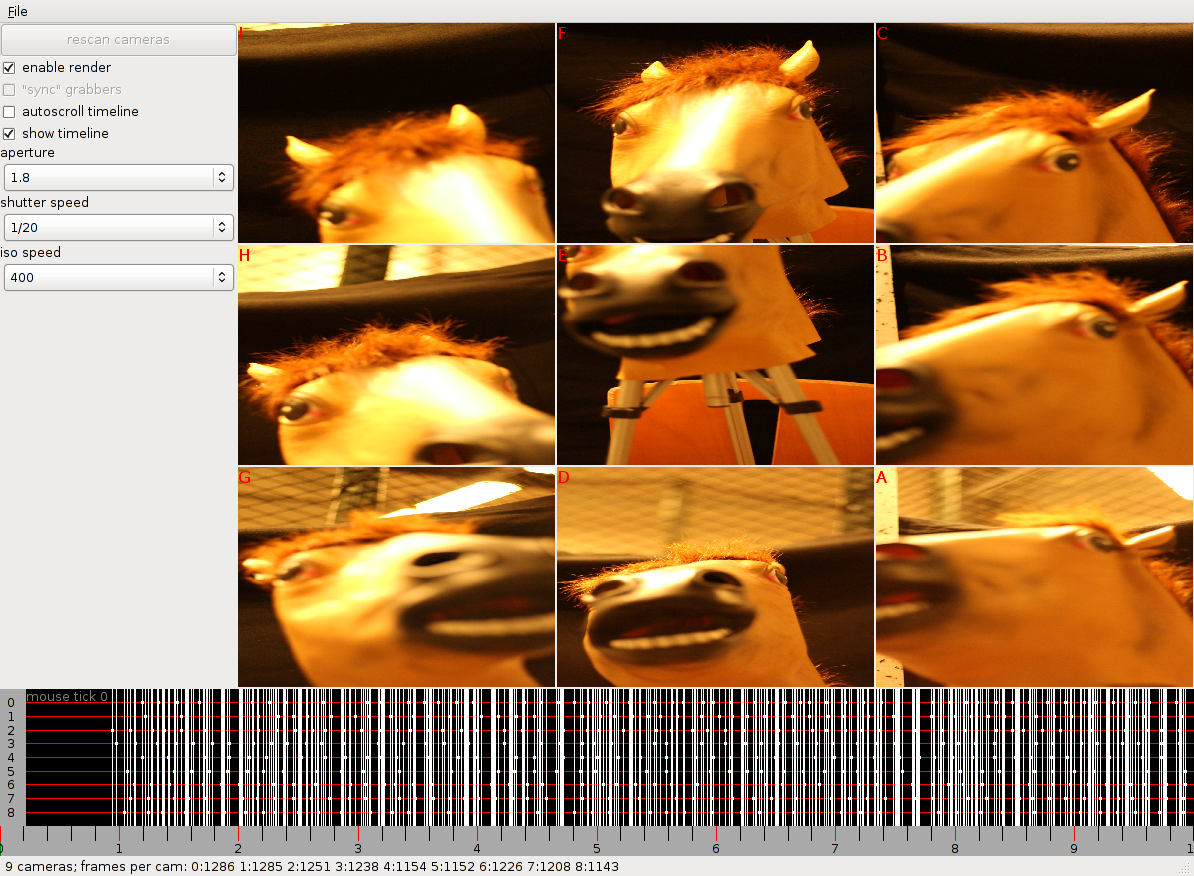
\includegraphics[width=0.8\textwidth]{gphotogrid}
	\begin{itemize}
		\item A great aid in aiming the rig as a whole
		\item Individual orientations with the viewfinders though
	\end{itemize}
\end{frame}

%%%%%%%%%%%%%%%%%%%%%%%%%%%%%%%%%%%%%%%%%%%%%%%%%%%%%%%%%%%%%%%%%%%%%%%%%%%%%%%%%%%%%%%%%%%%%

\begin{frame}[fragile]{Control}
	\begin{columns}[c]
	\column{0.5\textwidth}
	\begin{itemize}
		\item Camera exposes parameters via USB
		\item Shutter speed, aperture, ...
		\item Mostly implemented in gphoto2 CLI
		\item Image download as soon as captured
		\item USB connection to remote trigger box
	\end{itemize}
	\column{0.5\textwidth}
	\begin{Verbatim}[fontsize=\scriptsize]
./forallp.sh \
	--set-config imageformat=RAW \
	--set-config imageformatsd=RAW \
	--set-config shutterspeed="1/100" \
	--set-config iso="100" \
	--set-config colorspace="sRGB" \
	--set-config picturestyle="Standard" \
	--set-config focusmode="One Shot" \
	--set-config aperture="11" \
	--set-config meteringmode="Evaluative" \
	--set-config drivemode="Single" \
	--set-config capturetarget="Memory card"
	\end{Verbatim}
	\end{columns}
\end{frame}

%%%%%%%%%%%%%%%%%%%%%%%%%%%%%%%%%%%%%%%%%%%%%%%%%%%%%%%%%%%%%%%%%%%%%%%%%%%%%%%%%%%%%%%%%%%%%

\begin{frame}{Experiments}
	\begin{columns}[c]
	\column{0.5\textwidth}
	\begin{itemize}
		\item Synch tests
		\item Sample scans
		\item A few reconstruction programs tested
		\item Numerous libraries and commercial tools reviewed
		% list some of the tools?
	\end{itemize}
	\column{0.5\textwidth}
	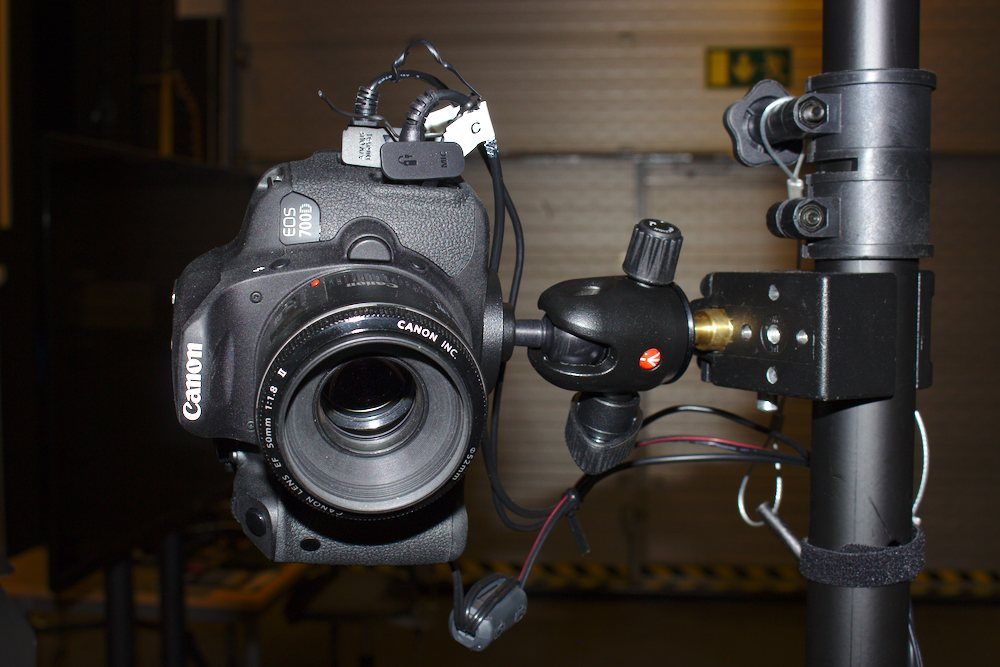
\includegraphics[width=\textwidth]{camconn}
	\end{columns}
\end{frame}

%%%%%%%%%%%%%%%%%%%%%%%%%%%%%%%%%%%%%%%%%%%%%%%%%%%%%%%%%%%%%%%%%%%%%%%%%%%%%%%%%%%%%%%%%%%%%

\begin{frame}{Source data}
\center
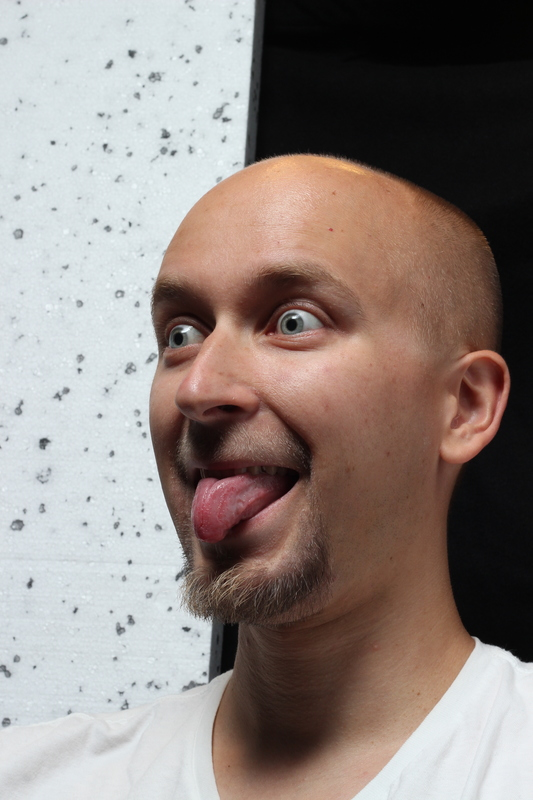
\includegraphics[width=0.3\textwidth]{arto-1}
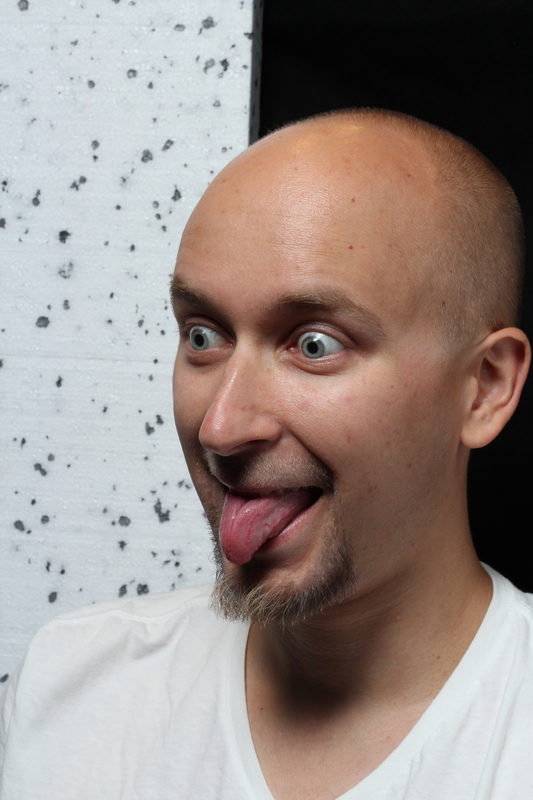
\includegraphics[width=0.3\textwidth]{arto-2}
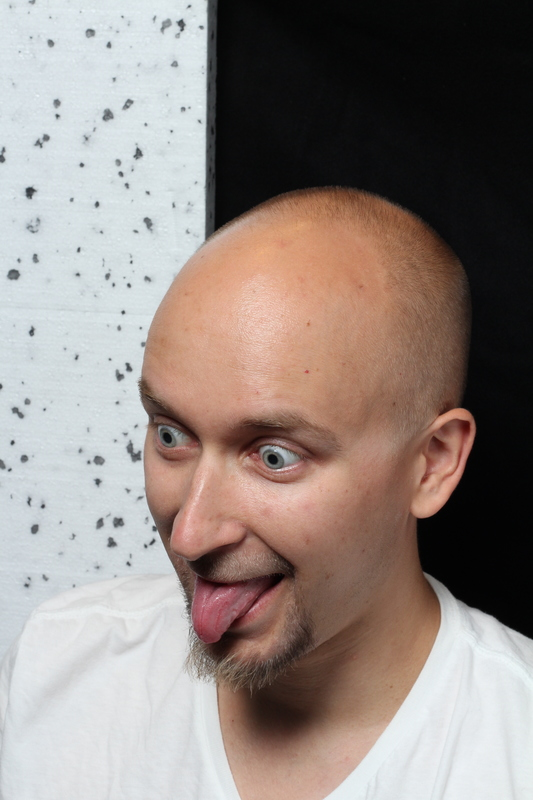
\includegraphics[width=0.3\textwidth]{arto-3}

18 Mpix per cam
\end{frame}

%%%%%%%%%%%%%%%%%%%%%%%%%%%%%%%%%%%%%%%%%%%%%%%%%%%%%%%%%%%%%%%%%%%%%%%%%%%%%%%%%%%%%%%%%%%%%

\begin{frame}{Output geometry}
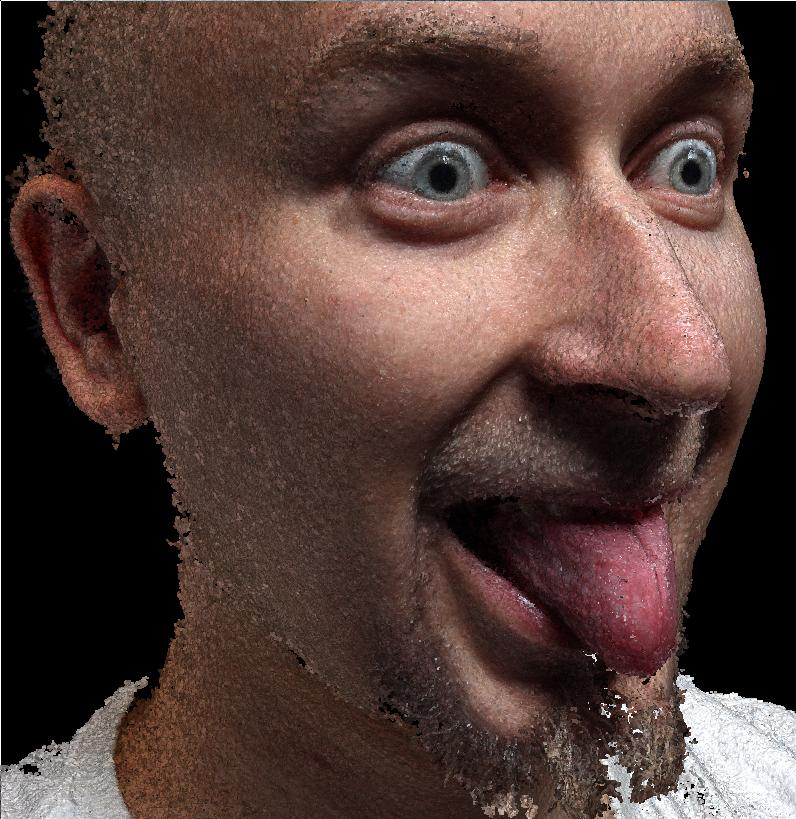
\includegraphics[width=0.5\textwidth]{photoscan-arto-dense}%
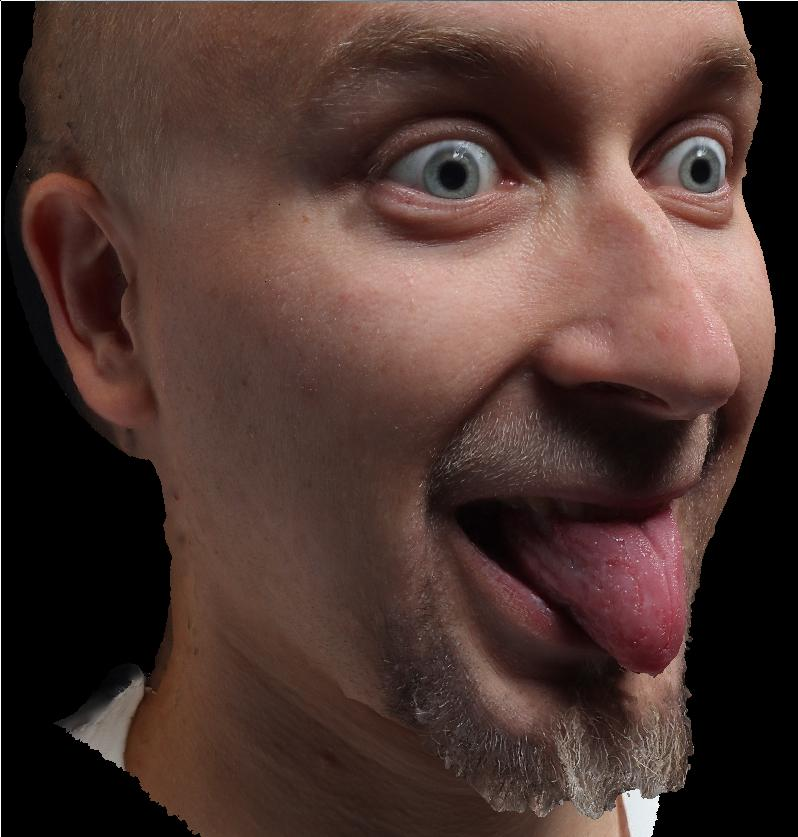
\includegraphics[width=0.5\textwidth]{photoscan-arto-textured}

1-5M points
\end{frame}

%%%%%%%%%%%%%%%%%%%%%%%%%%%%%%%%%%%%%%%%%%%%%%%%%%%%%%%%%%%%%%%%%%%%%%%%%%%%%%%%%%%%%%%%%%%%%

\begin{frame}{Textures}
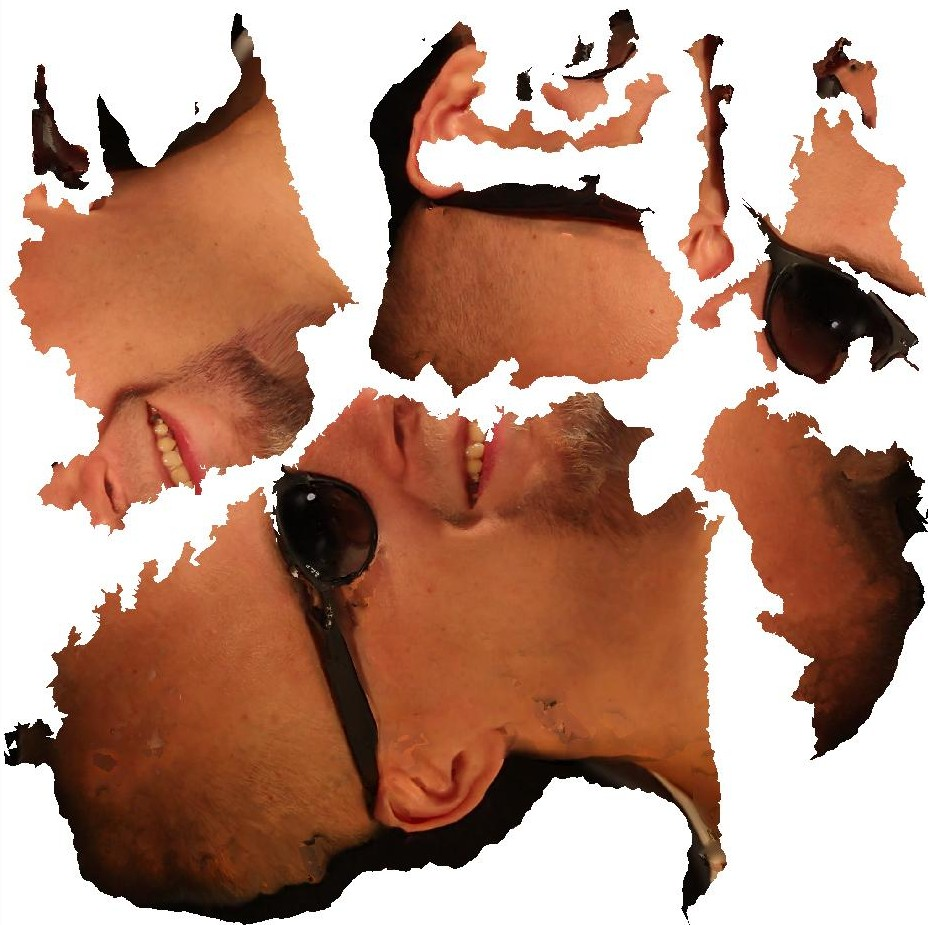
\includegraphics[width=0.5\textwidth]{artoglassuvgeneric}%
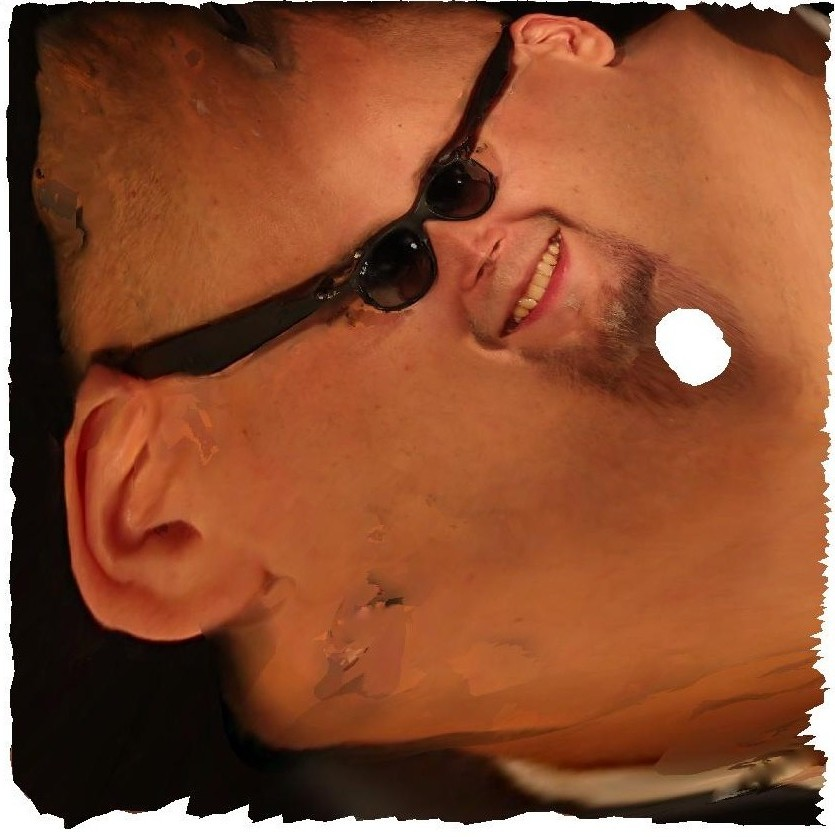
\includegraphics[width=0.5\textwidth]{artoglassuvspherical}
\end{frame}

%%%%%%%%%%%%%%%%%%%%%%%%%%%%%%%%%%%%%%%%%%%%%%%%%%%%%%%%%%%%%%%%%%%%%%%%%%%%%%%%%%%%%%%%%%%%%

\begin{frame}{Hand}
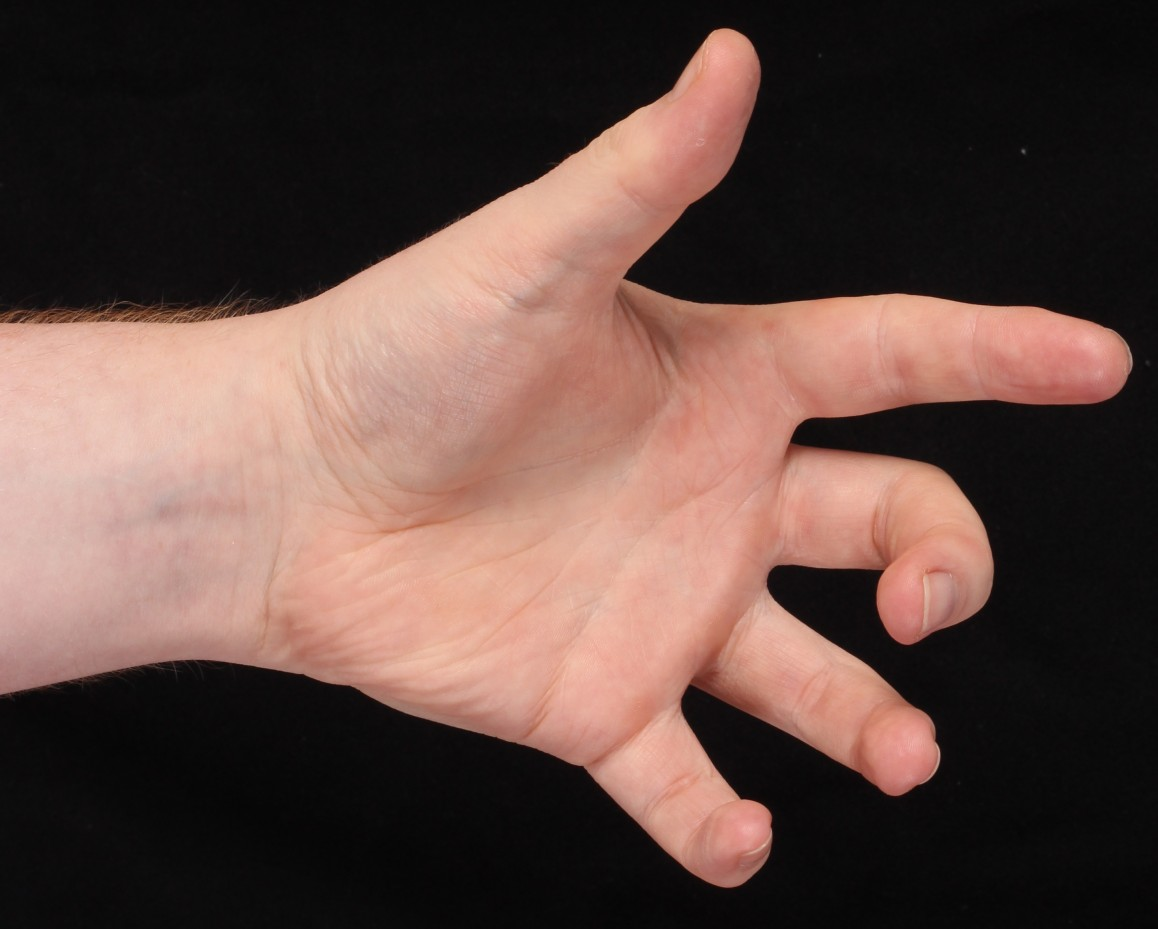
\includegraphics[height=0.5\textheight]{handorig}%
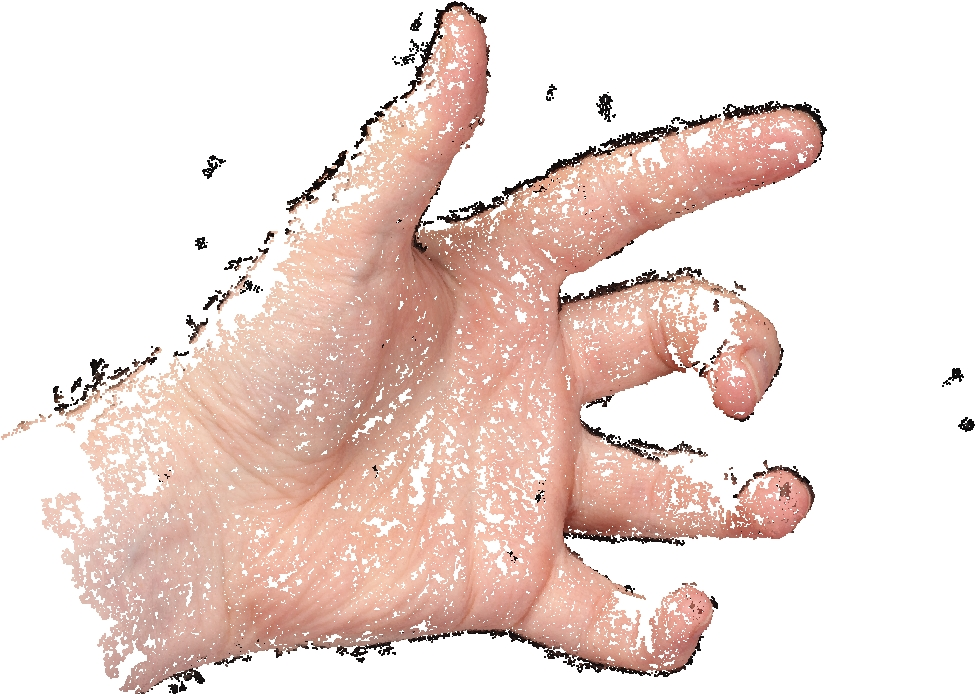
\includegraphics[height=0.5\textheight]{handreconst}

Occlusion issues
\end{frame}

%%%%%%%%%%%%%%%%%%%%%%%%%%%%%%%%%%%%%%%%%%%%%%%%%%%%%%%%%%%%%%%%%%%%%%%%%%%%%%%%%%%%%%%%%%%%%

\begin{frame}{Legos}
\center
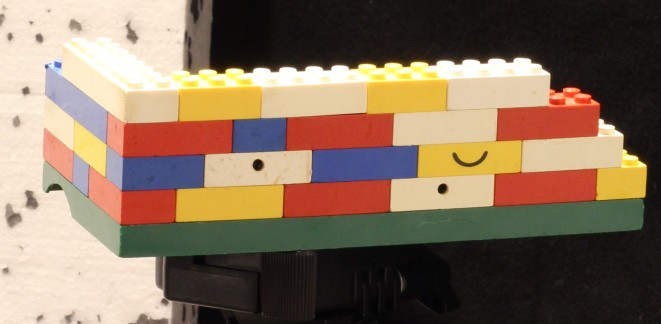
\includegraphics[width=0.6\textwidth]{legosorig}\\
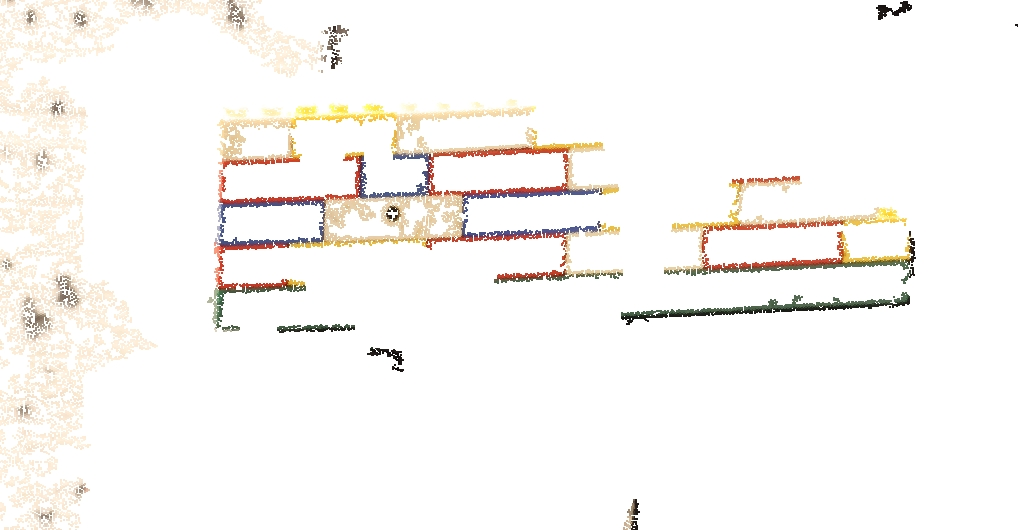
\includegraphics[width=0.6\textwidth]{legosreconst}

No texture
\end{frame}

%%%%%%%%%%%%%%%%%%%%%%%%%%%%%%%%%%%%%%%%%%%%%%%%%%%%%%%%%%%%%%%%%%%%%%%%%%%%%%%%%%%%%%%%%%%%%

\begin{frame}{Rubber mask}
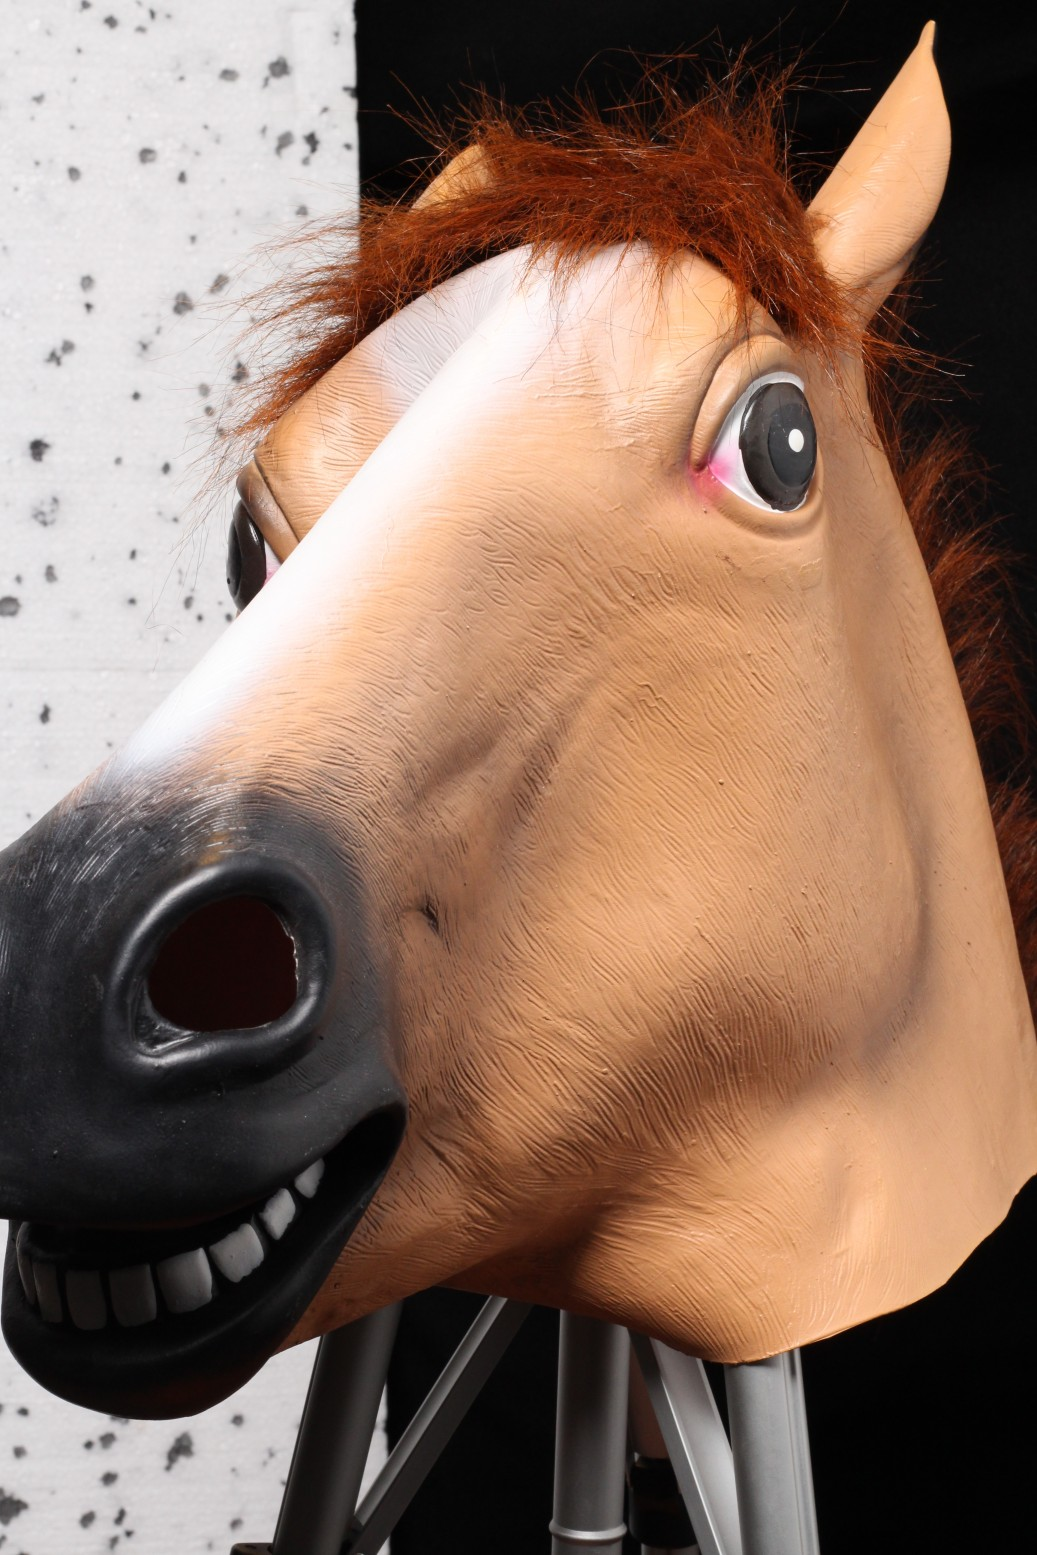
\includegraphics[height=0.6\textheight]{horseorig}
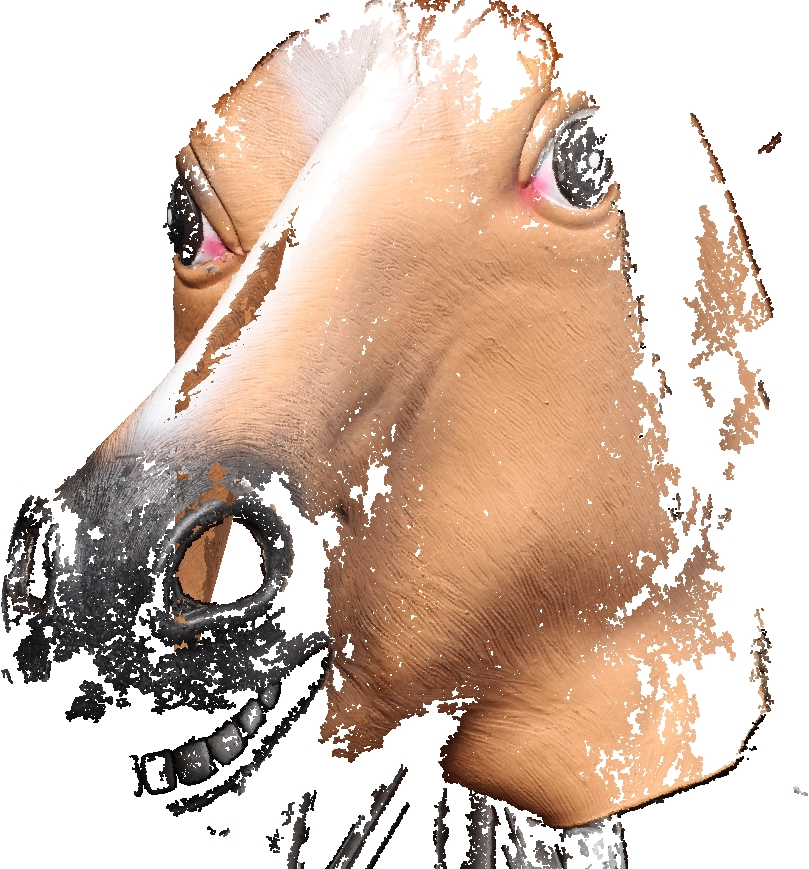
\includegraphics[height=0.6\textheight]{horsereconst}
\center

No texture
\end{frame}

%%%%%%%%%%%%%%%%%%%%%%%%%%%%%%%%%%%%%%%%%%%%%%%%%%%%%%%%%%%%%%%%%%%%%%%%%%%%%%%%%%%%%%%%%%%%%

\begin{frame}{Level of detail}
\center 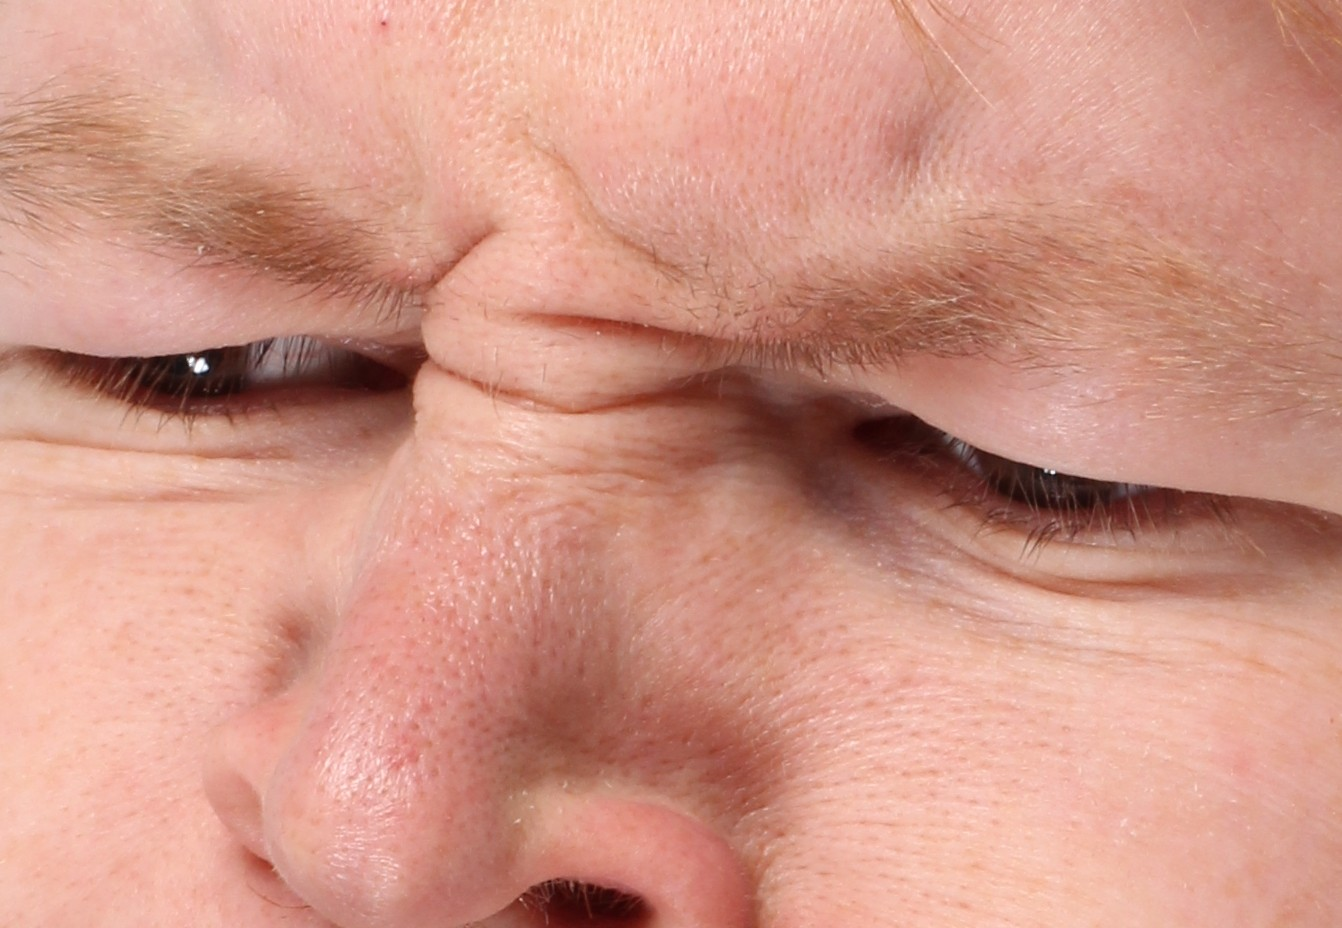
\includegraphics[width=0.7\textwidth]{soodaheadorigclose}\\
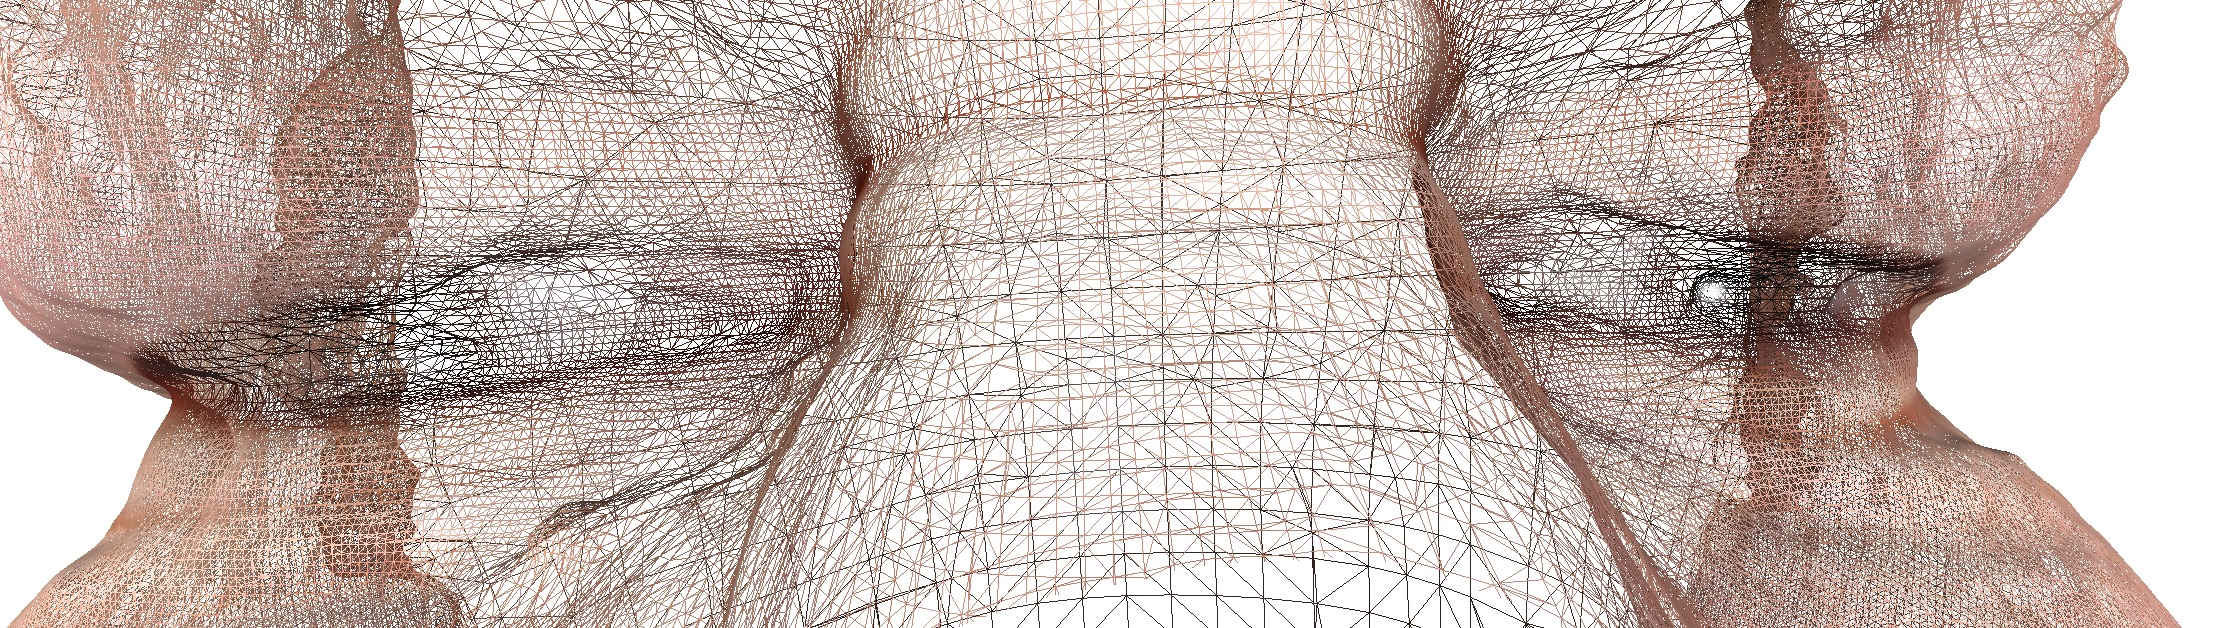
\includegraphics[width=0.7\textwidth]{soodaheadreconsteyeswire}
\end{frame}

%%%%%%%%%%%%%%%%%%%%%%%%%%%%%%%%%%%%%%%%%%%%%%%%%%%%%%%%%%%%%%%%%%%%%%%%%%%%%%%%%%%%%%%%%%%%%

\begin{frame}{Issues}
	\begin{itemize}
		\item Video synchronization
		\item Light requirements
		\item Post processing
		\item Camera quirks
	\end{itemize}
\end{frame}

%%%%%%%%%%%%%%%%%%%%%%%%%%%%%%%%%%%%%%%%%%%%%%%%%%%%%%%%%%%%%%%%%%%%%%%%%%%%%%%%%%%%%%%%%%%%%

\begin{frame}{Future work}
	\begin{columns}[c]
	\column{0.5\textwidth}
	\begin{itemize}
		\item (Actually use it)
		\item Reproduce state-of-the-art
		\item Mesoscopic face geometry
	\end{itemize}
	\column{0.5\textwidth}
	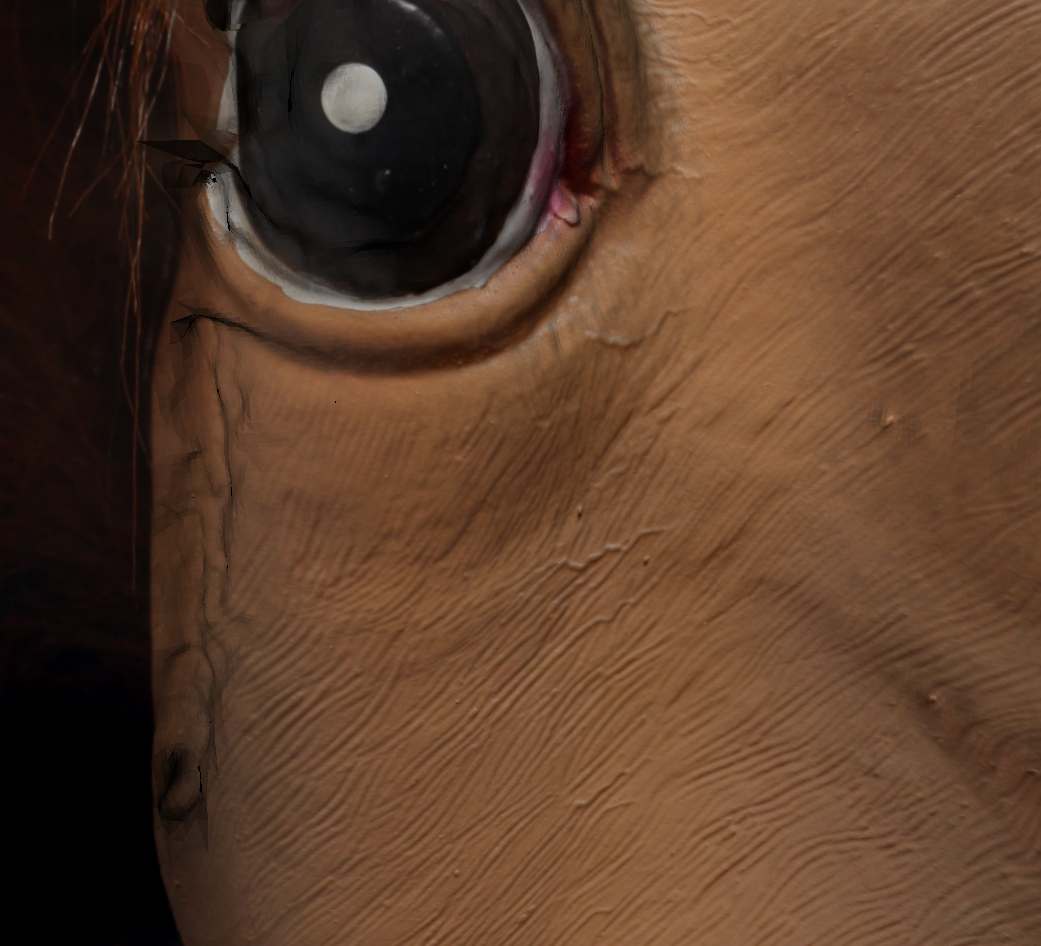
\includegraphics[width=\textwidth]{horseclose-tex}
	\end{columns}
\end{frame}

%%%%%%%%%%%%%%%%%%%%%%%%%%%%%%%%%%%%%%%%%%%%%%%%%%%%%%%%%%%%%%%%%%%%%%%%%%%%%%%%%%%%%%%%%%%%%

\begin{frame}{Conclusion}
	\center 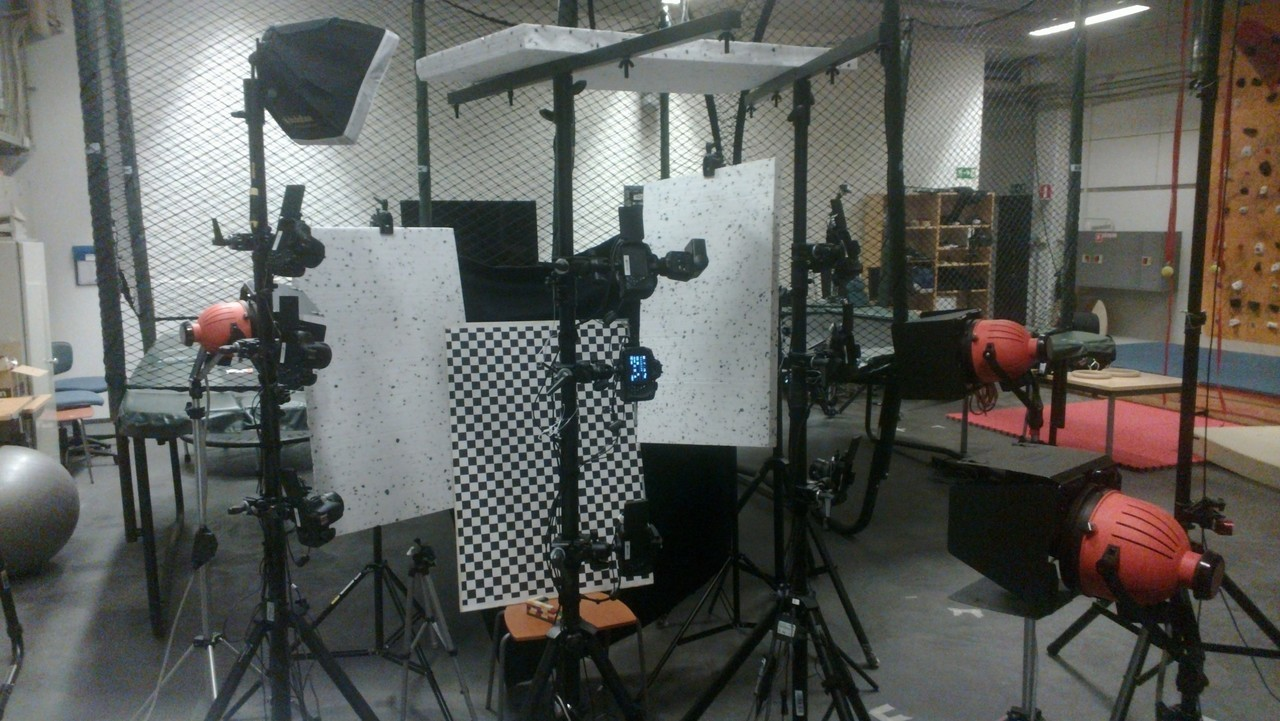
\includegraphics[width=0.6\textwidth]{totalsetup}
	\begin{itemize}
		\item Background and feasibility study $\Rightarrow$ built reconstruction rig
		\item Sub-millimeter-scale content
		\item Data needs post-processing
		\item Future work: actually use it
	\end{itemize}
\end{frame}


%%%%%%%%%%%%%%%%%%%%%%%%%%%%%%%%%%%%%%%%%%%%%%%%%%%%%%%%%%%%%%%%%%%%%%%%%%%%%%%%%%%%%%%%%%%%%

\end{document}
